Le système est développé en utilisant les technologies suivantes :

\begin{itemize}
    \item \textbf{Backend} :
    \begin{itemize}
        \item \textbf{Laravel} : Pour la gestion des utilisateurs, des données et l’intégration des services de notification (e-mail, FCM).
        \item \textbf{Python} : Pour le traitement des données, l’intégration OCR (OpenCV, Tesseract), et la communication avec les services de capture et d’analyse d’image.
    \end{itemize}
    
    \item \textbf{Frontend} :
    \begin{itemize}
        \item \textbf{React} : Pour l’interface web, permettant une visualisation interactive des données des patients et la gestion des alertes.
        \item \textbf{Flutter} : Pour l’application mobile, permettant au personnel médical de recevoir des notifications et d’accéder aux données des patients en temps réel.
    \end{itemize}
    
    \item \textbf{Base de données} :
    \begin{itemize}
        \item \textbf{MySQL} : Pour le stockage des données des patients, des alertes et des historiques.
    \end{itemize}
    
    \item \textbf{Protocoles de communication} :
    \begin{itemize}
        \item \textbf{REST API} : Pour la communication entre le frontend, le backend et l’application mobile.
        \item \textbf{WebSockets} : Pour les notifications en temps réel.
    \end{itemize}
    
    \item \textbf{Autres outils} :
    \begin{itemize}
        \item \textbf{Docker} : Pour la conteneurisation et le déploiement facile de l’application.
        \item \textbf{Git} : Pour le contrôle de version et la collaboration entre les membres de l’équipe.
        \item \textbf{Postman} : Pour tester les API REST.
        \item \textbf{Jest/PHPUnit} : Pour les tests unitaires en React et Laravel.
    \end{itemize}
\end{itemize}

\begin{figure}[H]
    \centering
    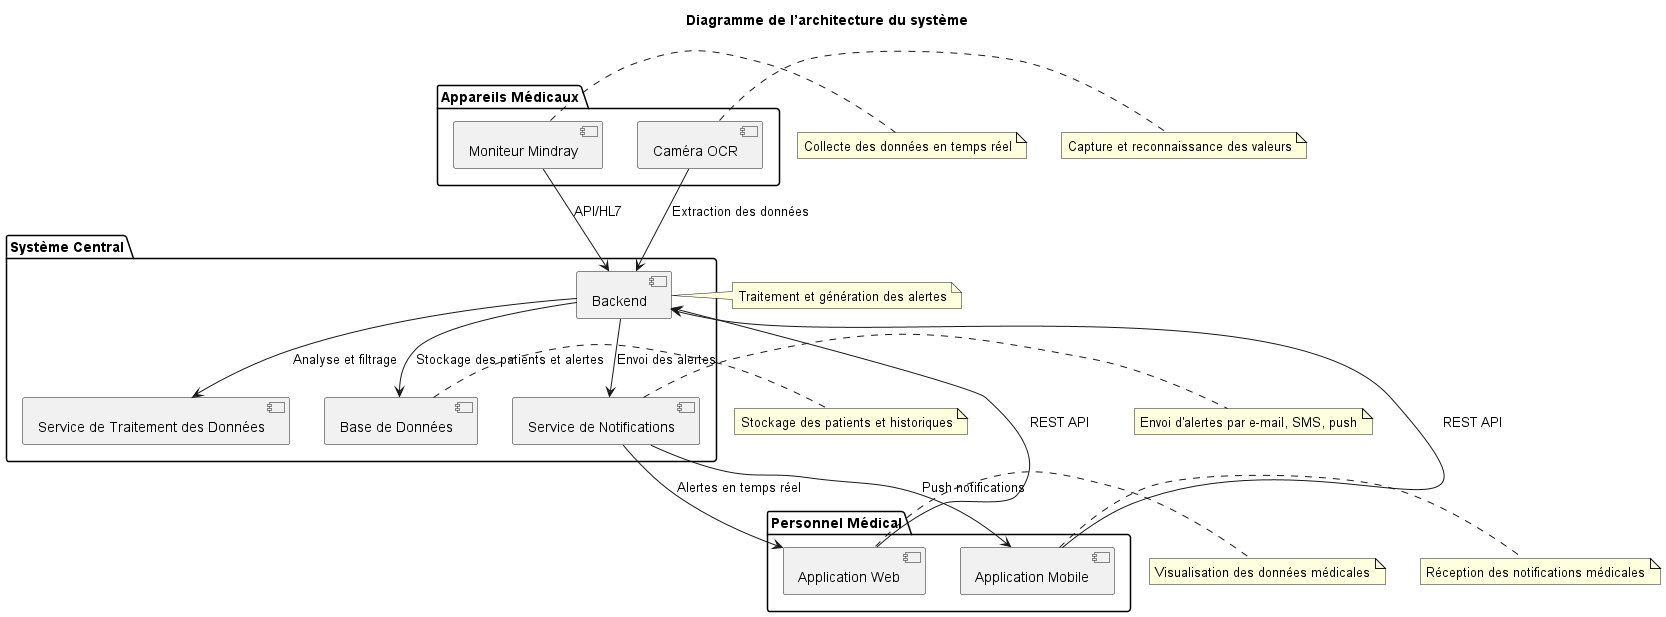
\includegraphics[width=1\textwidth]{chapter2/sections/diagrams/architecture.png}
    \caption{Diagramme de l’architecture du système}
    \label{fig:architecture}
\end{figure}